\chapter{Conformación de haz}\label{ch:beamforming}
\chapterquote{Never stopping. Never being satisfied. Never giving up. And if you keep pushing and keep moving forward, you're gonna go to places you never even dreamed of.}{Johnny Lawrence (Cobra Kai)}

\section{Introducción}\label{subc:beamforming_intro}
Al momento de realizar una comunicación inalámbrica uno de los aspectos que más contribuyen a la calidad del enlace es su dirección con respecto a la orientación de las antenas tanto del transmisor como del receptor. La capacidad de una antena de transformar en potencia eléctrica la energía recibida en forma de onda electromagnética en una cierta dirección viene caracterizada por su \textbf{patrón de radiación}. Este patrón caracteriza, también, el efecto contrario, es decir, la capacidad de una antena de convertir en energía radiada en una dirección particular la potencia eléctrica con la cual se la alimenta. Es por esto que a la hora de diseñar un enlace inalámbrico se busca que la dirección de mayor radiación de la antena transmisora y de la receptora, es decir, el \textbf{lóbulo principal} del patrón de radiación, coincida con la dirección del enlace, como se muestra en la Figura \ref{fig:beamforming_antenasorientadas}, de manera tal de lograr la mayor eficiencia en la transmisión de energía, lo cual repercute en una mejor relación señal a ruido (\textbf{SNR} por sus siglas en inglés) en la señal recibida.

\begin{figure}[ht]
    \centering
    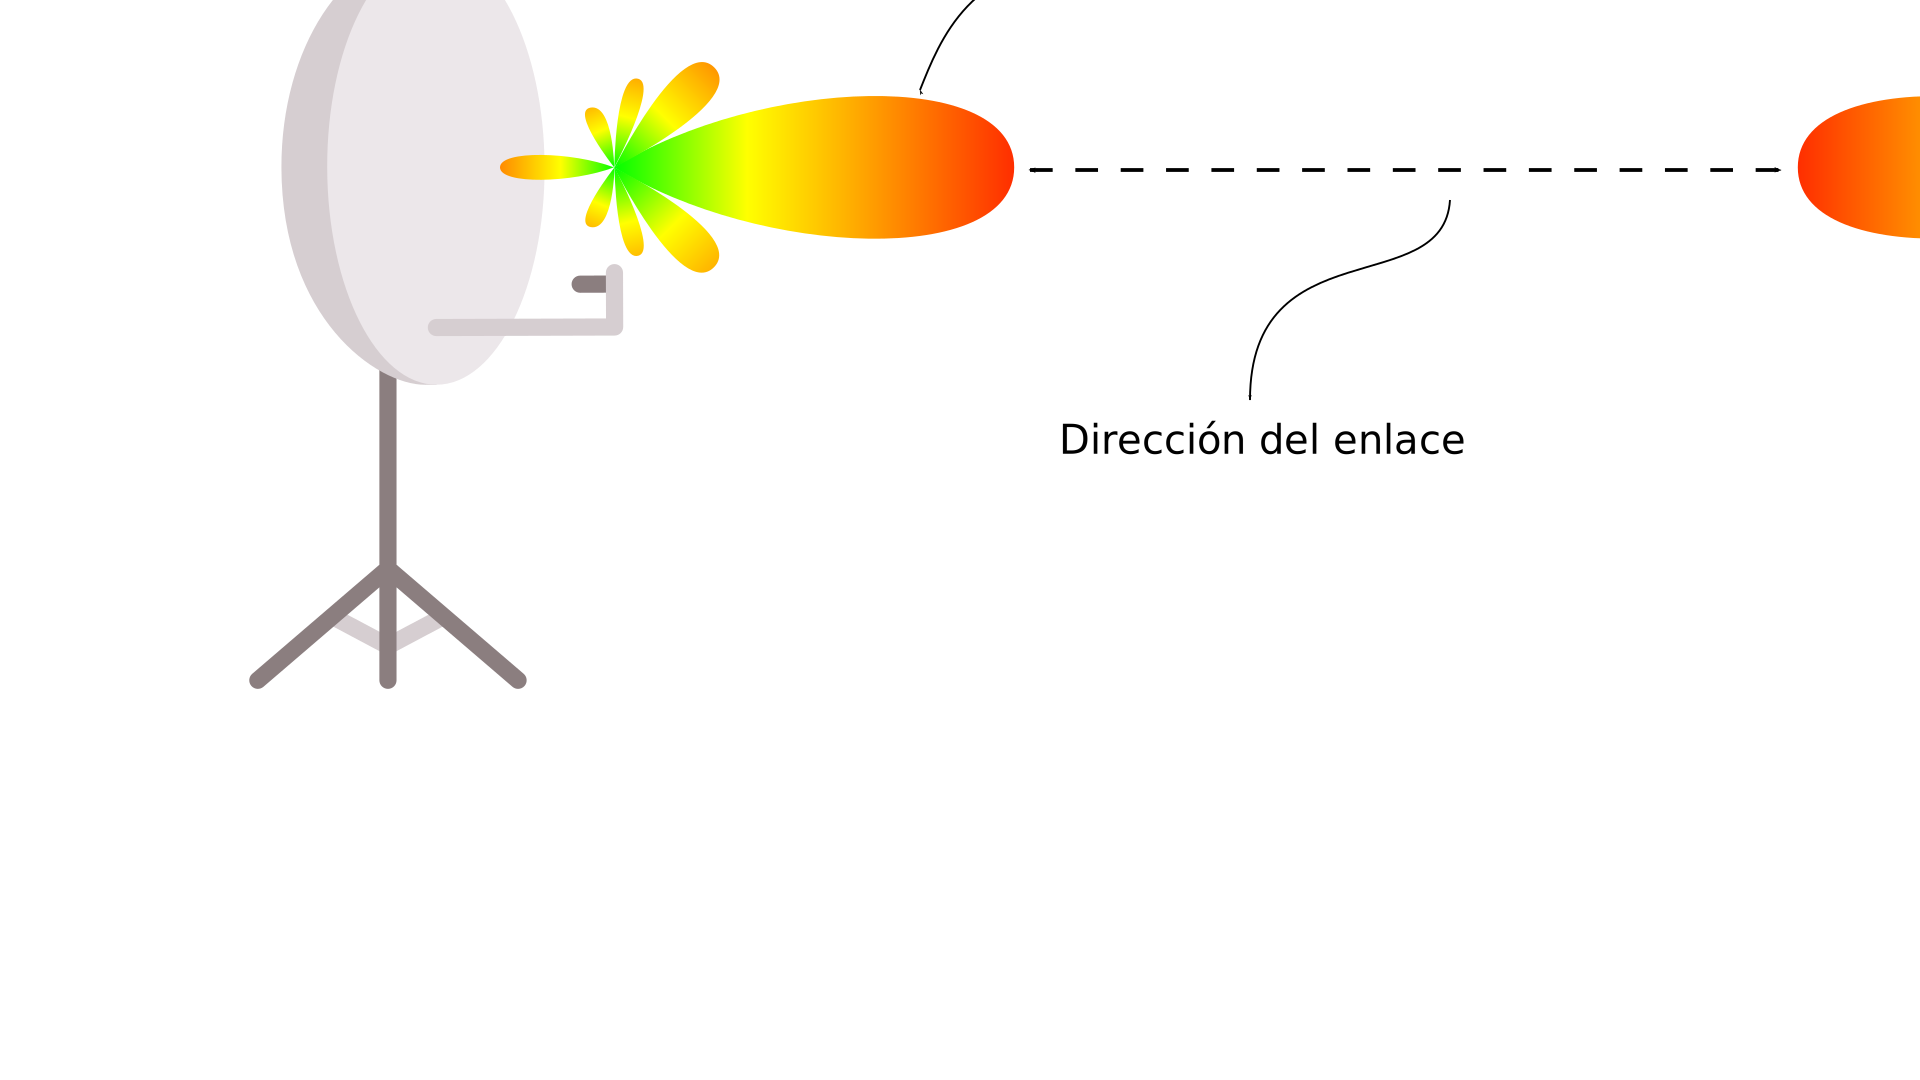
\includegraphics[width=1\linewidth]{images/02-Beamforming/antenasorientadas.png}
    \caption{Representación de un enlace punto a punto utilizando antenas parabólicas, indicando sus correspondientes patrones de radiación junto con sus lóbulos principales y secundarios.}
    \label{fig:beamforming_antenasorientadas}
\end{figure}

Lograr la mejor orientación de las antenas cuando el transmisor y el receptor se encuentran estáticos no conlleva mayores dificultades. Las complicaciones aparecen cuando uno de los dos o ambos se encuentran en movimiento. En este caso la solución que permite aumentar la eficiencia del enlace implica que al menos una de las antenas dirija su patrón de radiación de manera tal de poder hacer un seguimiento del objetivo con el cual se desea comunicar. Esto se puede lograr utilizando antenas móviles, como es el caso de las antenas parabólicas de las estaciones terrenas que se comunican con satélites de baja y media órbita, como las que se muestran en la Figura \ref{fig:beamforming_cordoba}.

\begin{figure}[ht]
    \centering
    \includegraphics[width=1\linewidth]{images/02-Beamforming/estacionterrenacordoba.jpg}
    \caption{Antenas parabólicas móviles de la estación terrena perteneciente al Centro Espacial Teófilo Tabanera \cite{bib:estacionterrena_cordoba}.}
    \label{fig:beamforming_cordoba}
\end{figure}

%En las comunicaciones satelitales para enlaces no geoestacionarios la transmisión de información se realiza entre un móvil (el satélite) y un transceptor que se encuentra fijo (la estación terrena).

Otra manera de lograr la orientación de los patrones de radiación de las antenas es mediante la técnica de \textbf{conformación de haz}, principal objeto de estudio de esta monografía. Esta técnica consiste en emular el comportamiento de una antena direccional mediante el sintetizado de patrones de radiación arbitrarios utilizando antenas estáticas. Esto se consigue utilizando un \textbf{arreglo de antenas en fase}, el cual consiste en un conjunto de antenas, generalmente idénticas, dispuestas en una disposición particular y con la capacidad de poder variar la fase relativa de la señal transmitida entre elementos, de manera tal de poder generar interferencias constructivas en la dirección en la que se quiere orientar el haz y destructivas en las direcciones desde las cuales se están recibiendo interferencias \cite{bib:Balanis_p303}.

La técnica de conformación de haz se puede aplicar a cualquier recepción o transmisión punto a punto de señales, sin embargo en este trabajo se orientará el estudio a la implementación de un conformador de haz para realizar comunicaciones con satélites de baja órbita. Para esto es necesario primero definir un sistema de coordenadas útil para describir la dirección de arribo de señales al momento de implementar una comunicación satelital. Este sistema es conocido por \textbf{coordenadas horizontales} y está definido por \cite{bib:MaralBousquet_p32}:

\begin{itemize}
    \item \textbf{Azimut:} es el ángulo tomado sobre el plano horizontal de la estación terrena midiendo desde el norte hacia la proyección de la dirección del satélite sobre el mismo plano en sentido horario. A lo largo de este trabajo se lo indicará con la letra griega $\varphi$.
    \item \textbf{Elevación:} es el ángulo formado entre la dirección del satélite y el plano horizontal. A lo largo de este trabajo se lo indicará con la letra griega $\theta$.
\end{itemize}

En la Figura \ref{fig:beamforming_lookangles} se muestra un esquema de este sistema de coordenadas.

\begin{figure}[ht]
    \centering
    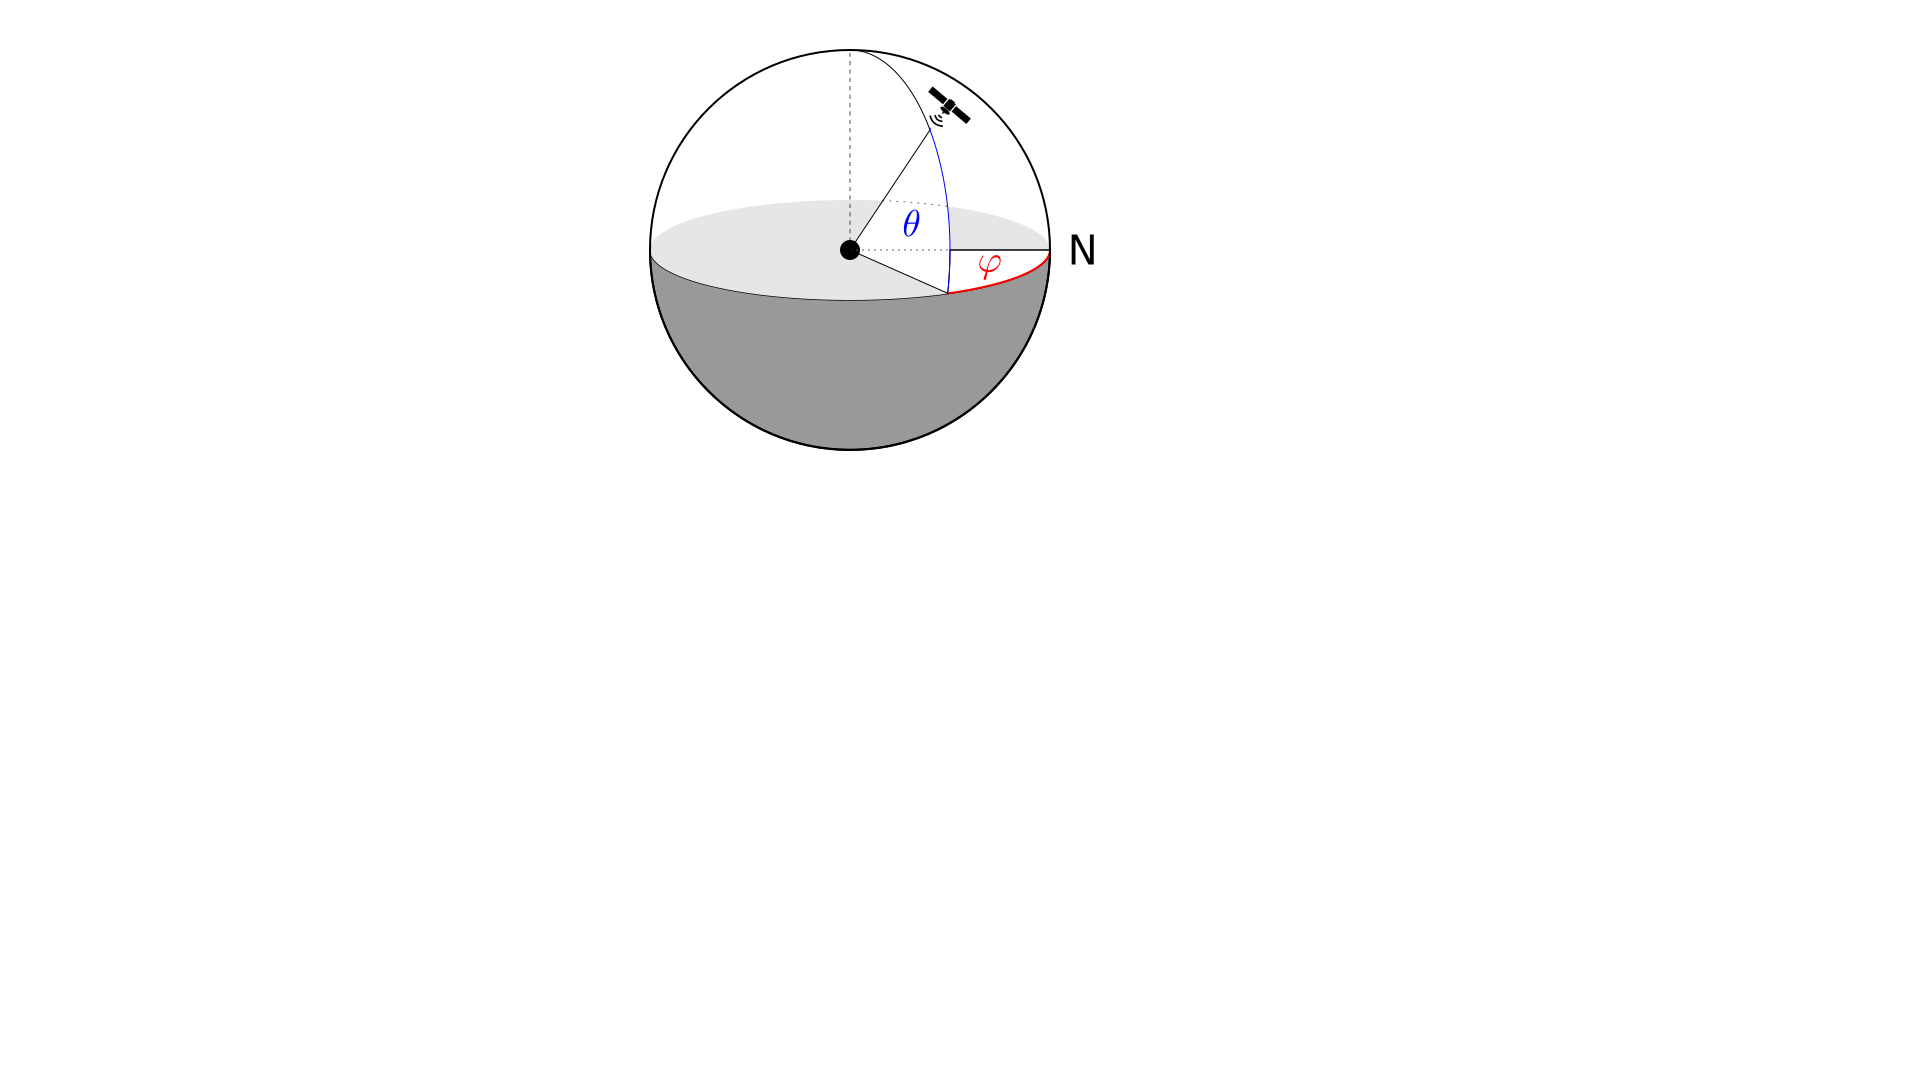
\includegraphics[width=0.7\linewidth]{images/02-Beamforming/lookangles.png}
    \caption{Sistema de coordenadas horizontales para comunicaciones satelitales.}
    \label{fig:beamforming_lookangles}
\end{figure}

Para comenzar a explicar en qué consiste la técnica de conformación de haz consideremos que tenemos un conjunto de antenas idénticas dispuestas sobre una línea y equidistantes unas de otras, a las cuales les llega un frente de onda con un cierto ángulo $\theta$ con respecto a la vertical, como se muestra en la Figura \ref{fig:beamforming_caso1d}.

\begin{figure}[ht]
    \centering
    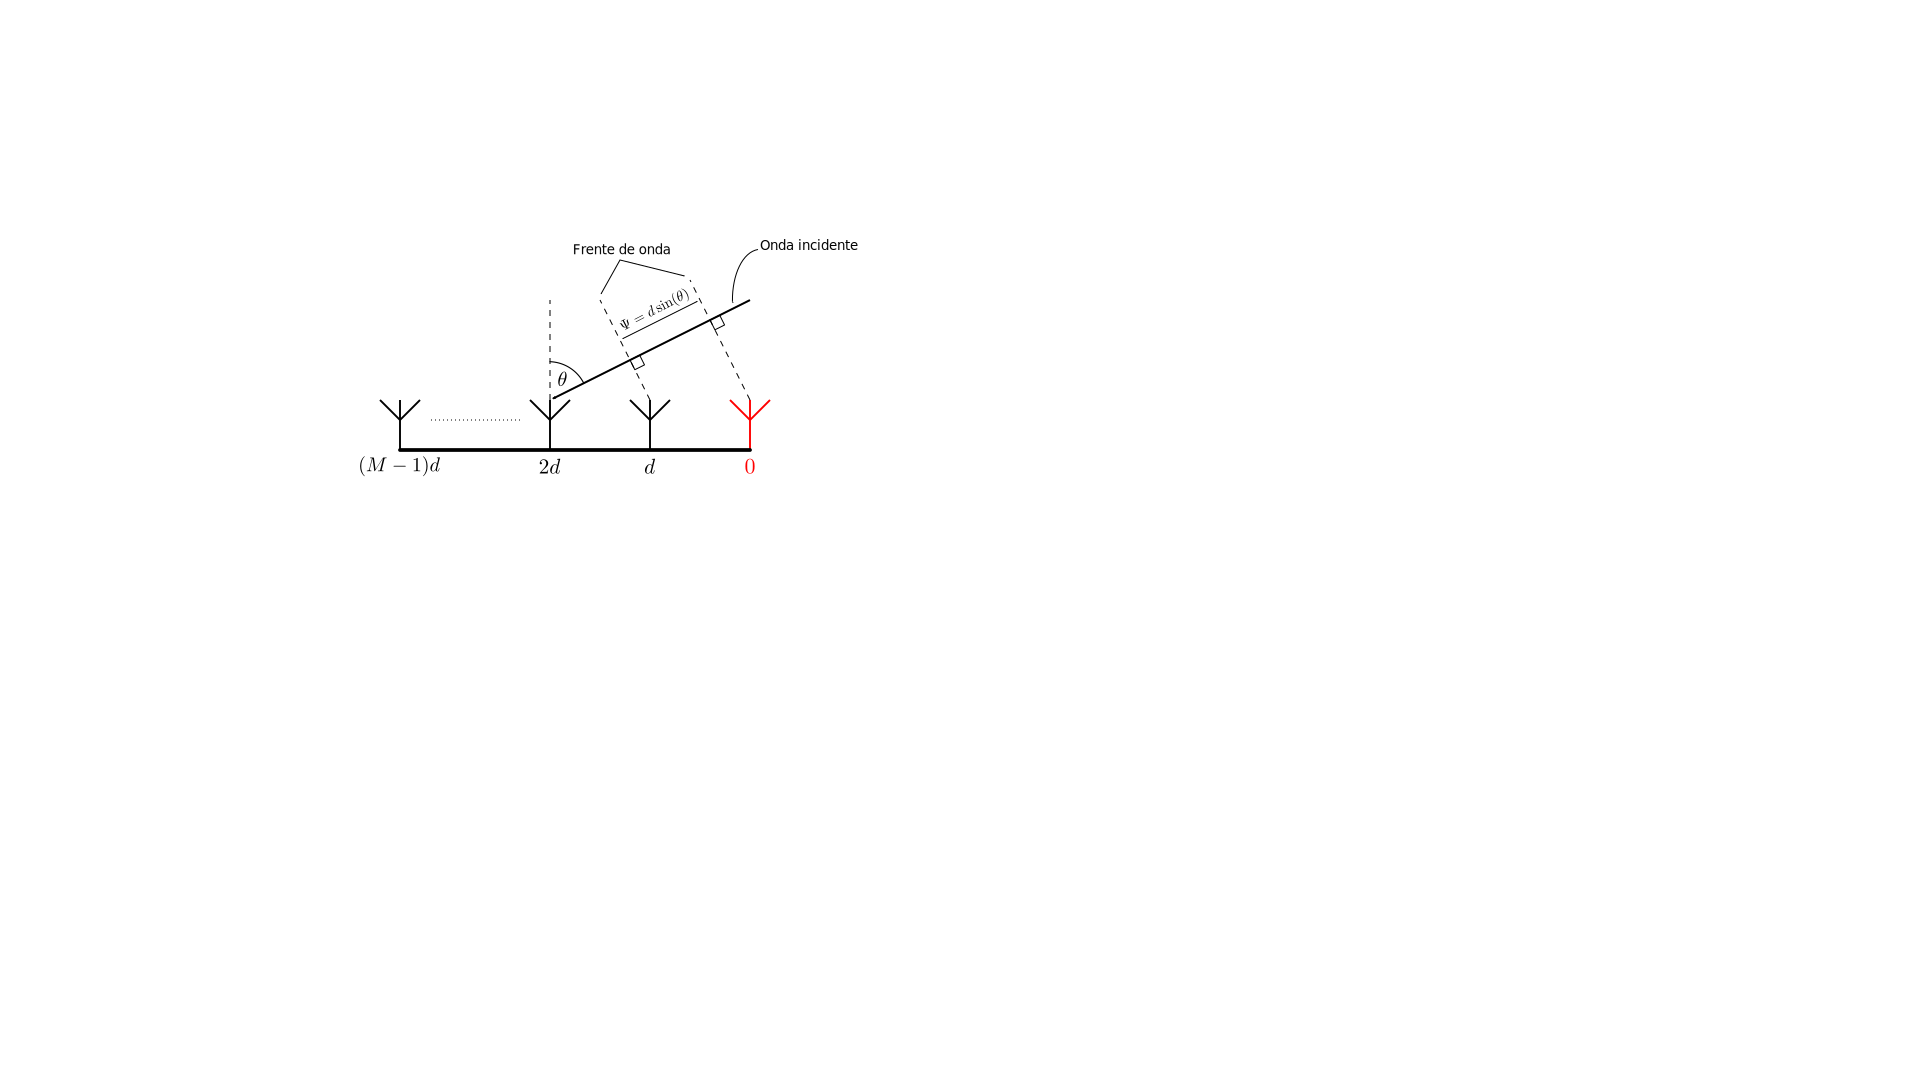
\includegraphics[width=0.8\linewidth]{images/02-Beamforming/caso1d.png}
    \caption{Frente de onda plano arribando a un arreglo lineal de antenas. Se indica en rojo el elemento de referencia, en el cual se considera que la señal arribante tiene fase nula.}
    \label{fig:beamforming_caso1d}
\end{figure}

Considerando que la señal proviene desde una distancia lejana (comparada con el tamaño del arreglo de antenas) podemos afirmar con gran precisión que el frente de onda que llega al arreglo de antenas es plano. La dirección de arribo de la señal, o \textbf{DOA} por sus siglas en inglés, en este caso definida únicamente por el ángulo $\theta$, provoca que el frente de onda recorra distintas distancias al llegar a cada elemento del arreglo, y esa diferencia en las distancias generan un desfasaje en la señal recibida por cada receptor. Por ende, teniendo en cuenta que la separación entre elementos del arreglo es la misma y que el frente de onda se lo puede considerar como plano, y eligiendo convenientemente al primer elemento del arreglo al cual llega el frente de onda como elemento de referencia, podemos obtener la diferencia de camino recorrido por la señal transmitida al llegar a cada receptor haciendo:

\begin{equation}
    \Psi_m = m\cdot d\sin(\theta),\quad m=0,1,2,...,(M-1),
\end{equation}
siendo $d$ la separación de elementos y $M$ la cantidad de elementos en el arreglo.

La forma de onda de una onda viajera en campo lejano recibida por un receptor puntual, considerando un transmisor también puntual e isotrópico, puede ser expresada por la magnitud de su campo eléctrico como \cite{bib:2decadesp69}:

\begin{equation}
    E(\bar{r},t)=s(t)e^{j(\omega_p t - \bar{k}\cdot\bar{r})},
\end{equation}
siendo:

\begin{itemize}
    \item $\bar{r}$: el vector que une al transmisor con el receptor,
    \item $s(t)$: la señal transmitida en función del tiempo,
    \item $\omega_p=2\pi f_p$: la frecuencia angular de la portadora,
    \item $\bar{k}$: el vector de onda, con $|\bar{k}|=\frac{2\pi}{\lambda_p}$,
    \item ${\lambda_p}$: la longitud de onda de la portadora.
\end{itemize}

Considerando el mismo arreglo de antenas de la Figura \ref{fig:beamforming_caso1d} podemos expresar la onda recibida por el $m-\textrm{ésimo}$ elemento como

\begin{equation}
    E_m(\bar{r_m},t)=s(t)e^{j(\omega_p t - \bar{k}\cdot\bar{r_m})},\quad m=0,1,2,...,(M-1),
\end{equation}
siendo $\bar{r_m}$ el vector que une el transmisor con el $m-\textrm{ésimo}$ receptor.
Es necesario aclarar que para que esta expresión sea válida es necesario que se cumpla la condición de que la señal $s(t)$ sea de banda angosta \cite{bib:2decadesp70}, lo cual significa que su ancho de banda debe ser al menos uno o dos órdenes de magnitud menor a la frecuencia de portadora. Esto permite asumir que la envolvente de la onda transmitida no varía demasiado en el tiempo que le lleva al frente de onda alcanzar todos los elementos del arreglo, y en cambio se la puede considerar constante.

Por conveniencia para el resto del análisis se quitará el término $e^{j\omega_p t}$ correspondiente a la variación de la señal debido a la portadora para trabajar con la señal en banda base, la cual se denotará con la letra $x$. Si tomamos como referencia al primer elemento al cual le llega el frente de onda de la señal transmitida podemos considerar que la fase de la señal recibida por este es nula, y expresar al resto de las señales recibidas por los demás elementos en función de la señal de referencia como:

\begin{equation}
    x_m (\theta,t) =s(t) e^{-j\cdot m \cdot k \cdot d\sin(\theta)},\quad m=0,1,2,...,(M-1),
    \label{eq:beamforming_sample_ula_iso}
\end{equation}
donde se observa que la señal recibida por el $m-\textrm{ésimo}$ receptor difiere con respecto a las recibidas por el resto de los receptores únicamente en una fase, la cual además depende únicamente del ángulo de arribo $\theta$ y de la separación entre elementos $d$. Esto intuye a pensar que si se conocen estos dos parámetros (la dirección de arribo y la disposición en la que están dispuestas las antenas receptoras) se podría conocer fácilmente las fases relativas entre todas las señales, pudiendo así corregirlas y sumarlas de manera tal de poder aumentar la relación señal a ruido en la señal recibida por el conjunto de antenas. A esta técnica se la conoce como conformación de haz.

Más allá de que este análisis se hizo teniendo en cuenta muchas suposiciones y únicamente para el caso de una disposición de elementos del arreglo de antenas en una única dimensión, más adelante se mostrará que este mismo análisis vale para casos generales, particularmente con distintas disposiciones de arreglos de antenas en dos dimensiones. También el mismo análisis se puede aplicar para la transmisión direccional de señales utilizando arreglos de antenas, sin embargo ese análisis no es motivo de estudio de este trabajo.

A lo largo de este capítulo se desarrollará toda la teoría detrás de la conformación de haz, haciendo hincapié en los distintos tipos de técnicas que existen para su implementación, definiendo propiamente a los arreglos de antenas en fase y detallando los dos algoritmos de estimación de dirección de arribo que fueron de mayor importancia para la realización de este proyecto.



\section{Clasificación de conformadores de haz}

Según como se realice la implementación, los conformadores de haz pueden recibir distintas clasificaciones. Si se pone el foco en la manera de manipular las señales recibidas podemos distinguir entre los conformadores de haz analógicos y digitales \cite{bib:steiskalp107-108}. En el caso del conformador de haz analógico la señal que llega a cada elemento del arreglo de antenas pasa por un desfasador analógico que permite compensar las fases relativas de las señales generadas cuando el frente de onda llega con una cierta dirección a cada elemento. Luego de esto, se combinan todas las señales con un combinador de potencias y solo se digitaliza la salida de este. Si se cuentan con $M$ elementos en el arreglo, este método reduce la dimensión de la señal recibida de $M$ a 1, reduciendo también así gran parte de la información recibida y solo permitiendo la recepción en una única dirección. Además de corregir las fases de las señales recibidas se puede además variar las ganancias de cada elemento de manera tal de generar interferencias destructivas en las direcciones donde queremos eliminar cualquier tipo de interferencia. Un esquema de este conformador se muestra en la Figura \ref{fig:beamforming_analogbeamformer}, donde los pesos $w_n$ son los números complejos que multiplican la señal recibida por cada elemento del arreglo para compensar las fases relativas y generar ganancias nulas en las direcciones de interferencias, de manera tal de poder así sintetizar el correspondiente patrón de radiación.

\begin{figure}
    \centering
    \begin{subfigure}[b]{0.7\textwidth}
        \centering
        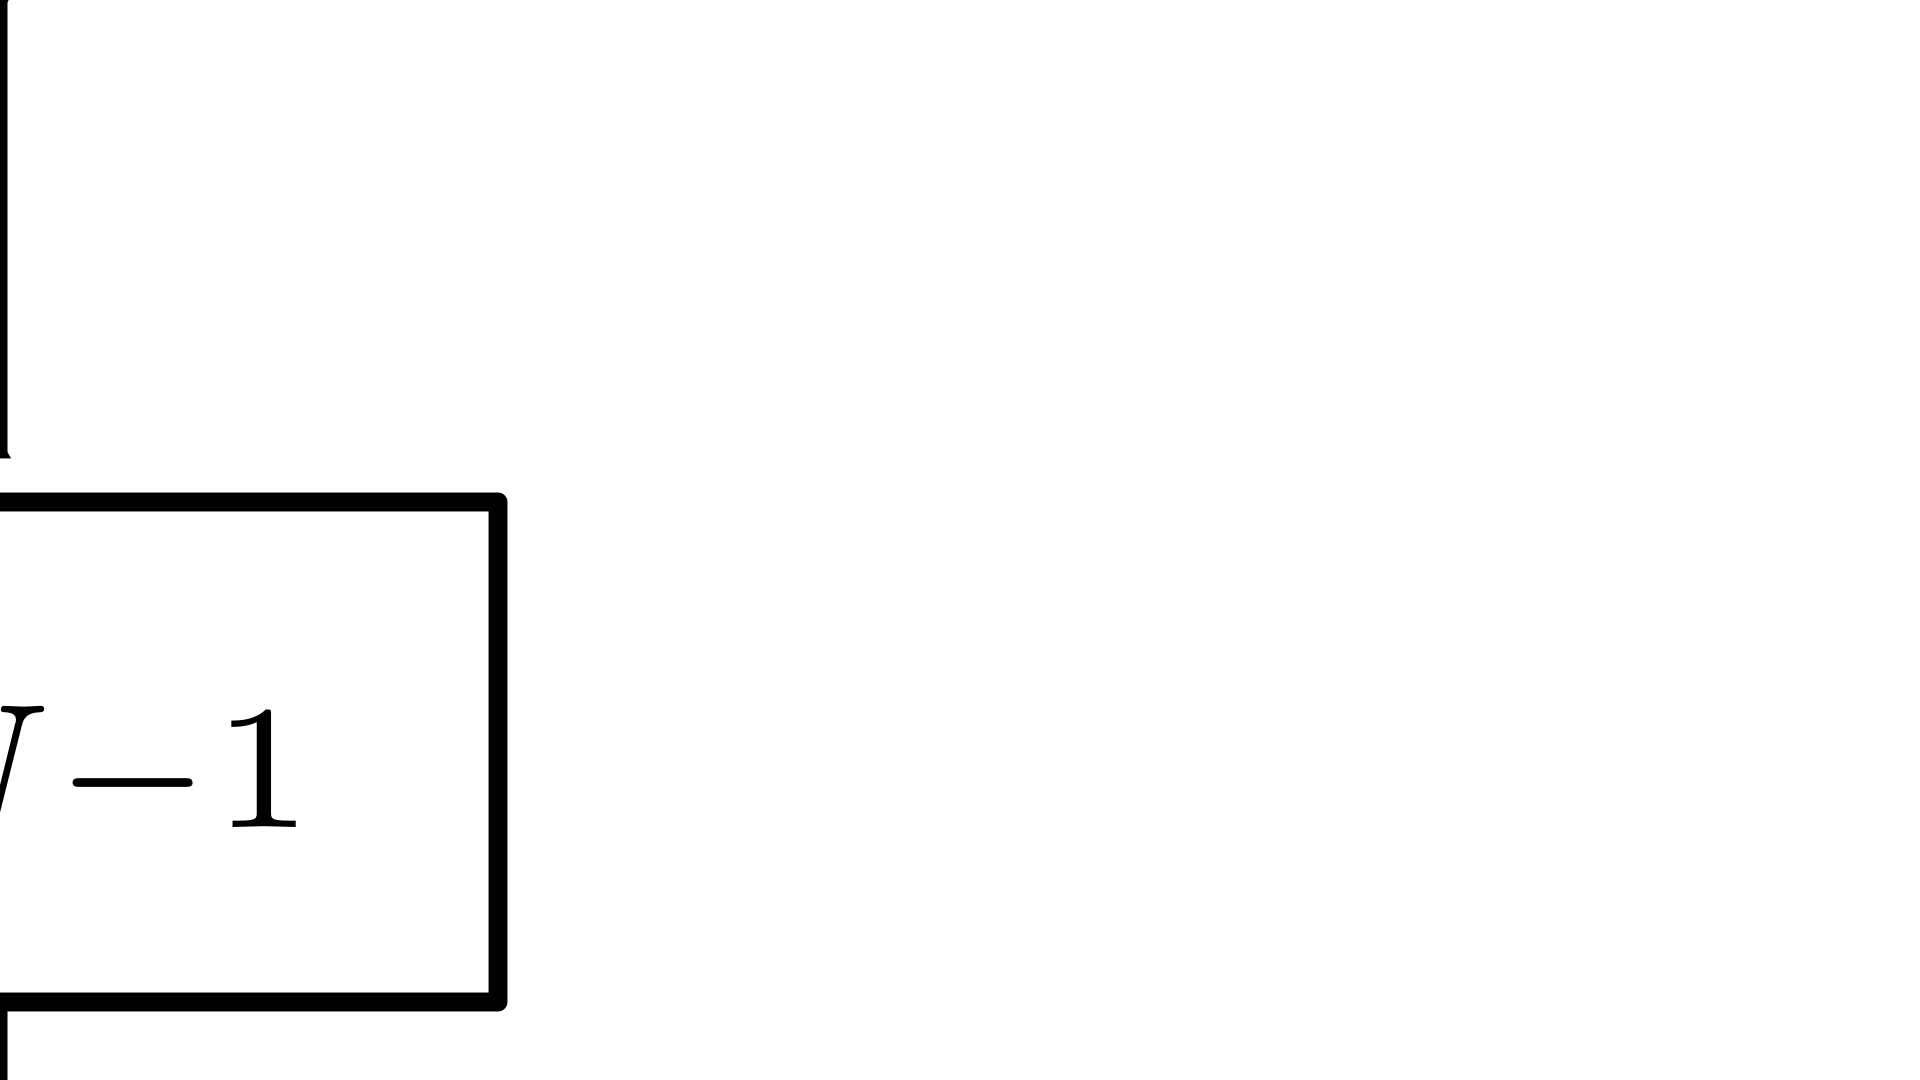
\includegraphics[width=\linewidth]{images/02-Beamforming/analogbeamformer.png}
        \caption{Conformador de haz analógico.}
        \label{fig:beamforming_analogbeamformer}
    \end{subfigure}
    \hfill
    \begin{subfigure}[b]{0.8\textwidth}
        \centering
        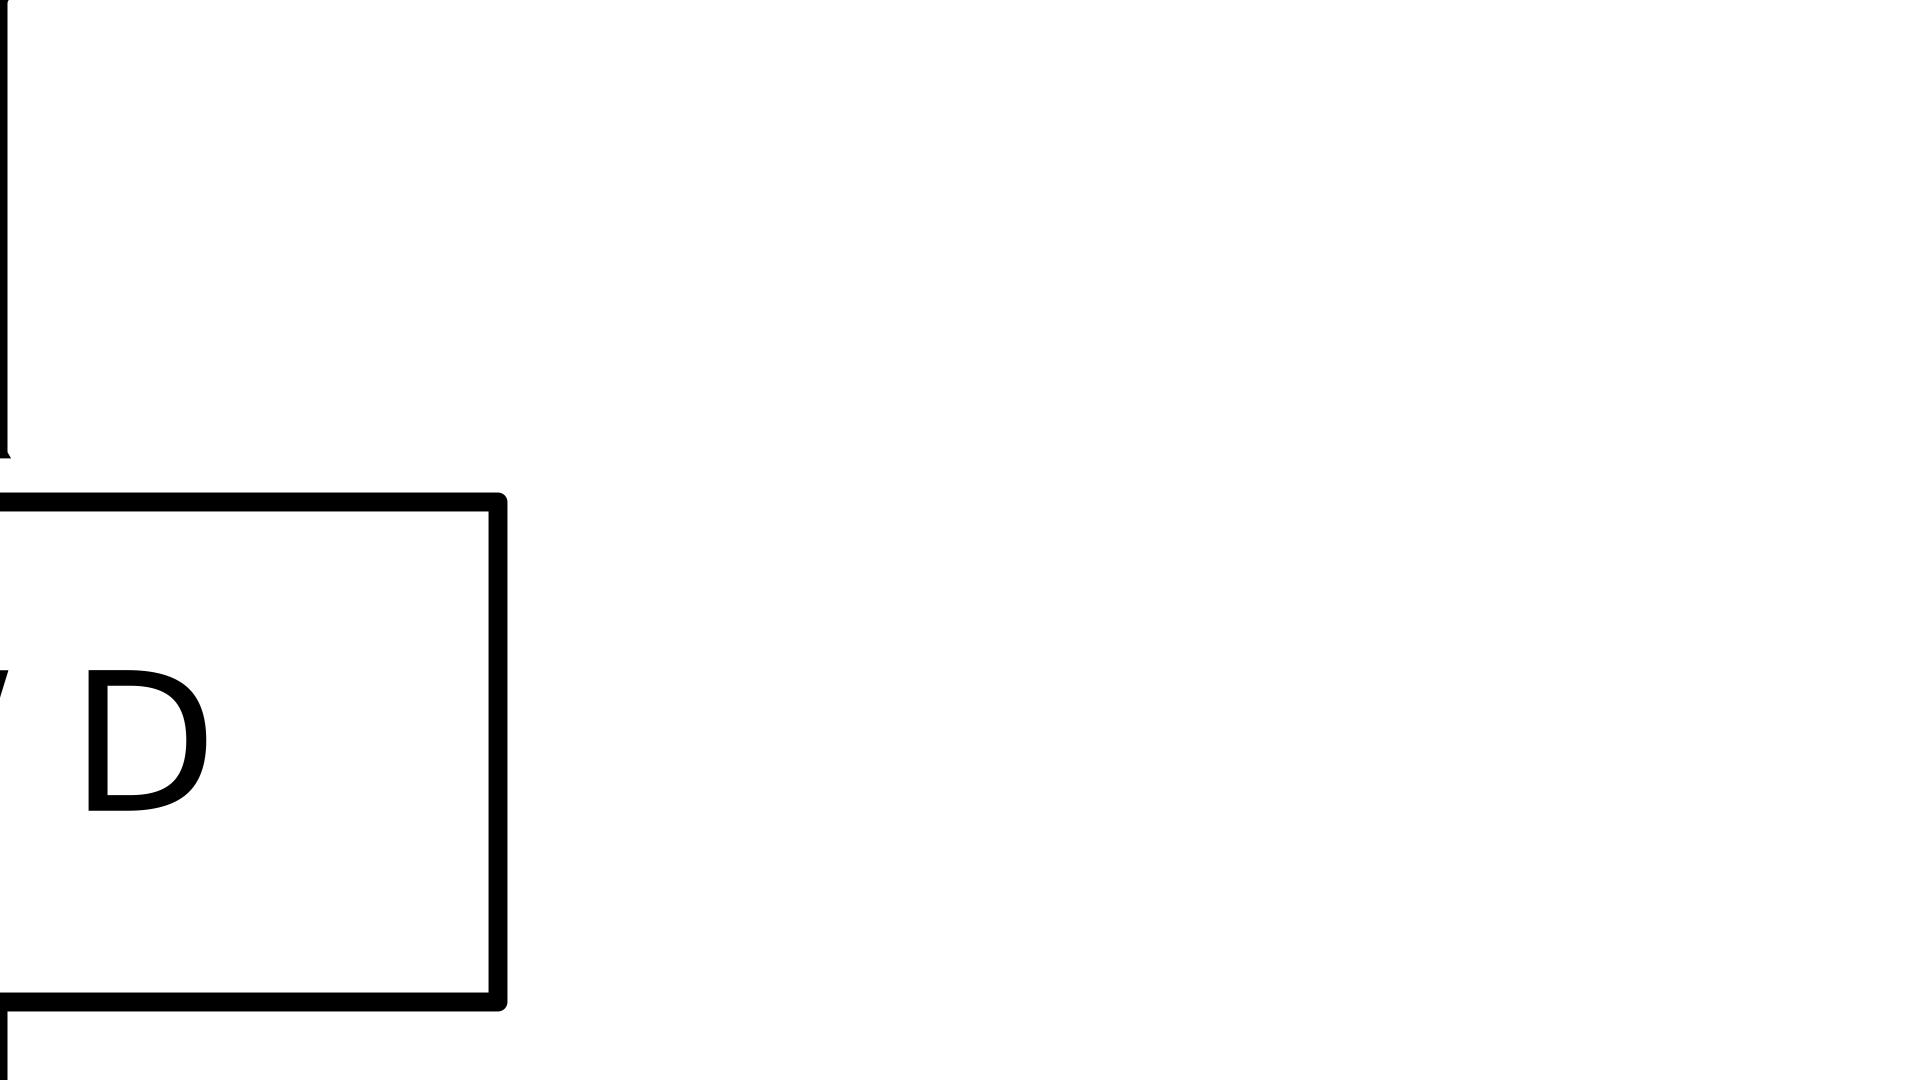
\includegraphics[width=\linewidth]{images/02-Beamforming/digitalbeamformer.png}
        \caption{Conformador digital de haz.}
        \label{fig:beamforming_digitalbeamformer}
    \end{subfigure}
    \caption{Clasificación de conformadores de haz según cómo manipulan la señal recibida.}
\end{figure}

En el conformador digital de haz las señales son muestreadas y digitalizadas para luego ser procesadas por un procesador digital. En este caso se preserva la información disponible manteniendo todas las señales recibidas por cada elemento. De esta manera la dimensión de la señal recibida se mantiene, lo cual brinda una gran flexibilidad para operar con las muestras recibidas, permitiendo obtener grandes prestaciones que no se encuentran disponibles en su contraparte analógica. Algunas de ellas son la capacidad de rechazar automáticamente las interferencias o de estimar automáticamente la dirección de arribo de las señales de interés, la posibilidad de generar múltiples haces con un único conformador, lo cual permite recibir señales en múltiples direcciones de arribo, la capacidad de realizar una calibración de las antenas por procesamiento o la posibilidad de incluir inteligencia artificial en la conformación de haz, tema en el cual se entrará un poco más en detalle en la Sección \ref{subc_smartbeamforming}.

Según la técnica utilizada, los conformadores de haces pueden también clasificarse en convencionales o adaptativos \cite{bib:digitalantennasp6}. En el caso de los conformadores de haz convencionales el array de pesos y fases relativas se encuentran fijos, lo cual no permite realizar una adaptación a cambios en el tiempo ya sea en la dirección de arribo de la señal u otros cambios que pueden ocurrir en las características del arreglo o en el medio de transmisión. En cambio los conformadores adaptativos utilizan las propiedades estadísticas de la señal y del medio para variar los desfasajes y los pesos del filtro adaptativo y así poder hacer seguimiento de señales y mejorar la SNR.

A lo largo de este trabajo se estudiará la implementación de un conformador digital de haz adaptativo.


\section{Arreglos de antenas en fase}\label{subc:beamforming_phasedarrays}

Los arreglos de antenas en fase consisten en un conjunto de antenas estacionarias (elementos) dispuestas en una distribución unidimensional o bidimensional y que utilizan un control de variación de fases o retrasos temporales en cada elemento para escanear un haz en una dirección dada en el espacio y un control de amplitudes para dar forma al patrón de radiación \cite{bib:phahandbook_p1}. Como ya se dijo, su principal uso se debe a la posibilidad que tienen de sintetizar un patrón de radiación direccional que puede ser dirigido electrónicamente.

La dimensión en la que están dispuestos los elementos del arreglo definen el direccionamiento que se le puede dar al haz sintetizado. En el caso de una disposición unidimensional solo se podrá dirigir el haz en función de la elevación, en cambio en disposiciones bidimensionales el haz se puede dirigir tanto en elevación como en azimut.

A primera vista pareciera ser que este tipo de antenas solo ofrece ventajas comparadas con las antenas de apertura fija. La relación de compromiso está en la dificultad de fabricación, ya que los arreglos de antenas en fase tienen complicaciones que no existen en otras antenas, como la necesidad de que no existan desfasajes en las conexiones entre los elementos o el problema del acoplamiento mutuo entre antenas debido a la poca separación que existe entre unas y otras.

\subsection{Tipos de arreglos}\label{subc:beamforming_phasedarraystipos}

A pesar de que los elementos de un arreglo de antenas en fase se pueden ubicar en cualquier disposición arbitraria, existen ciertas distribuciones que habilitan la utilización de técnicas que son de gran utilidad al trabajar con la conformación de haz, como lo es la posibilidad de utilizar algoritmos de estimación de dirección de arribo. Generalizando la expresión de la Ecuación \ref{eq:beamforming_sample_ula_iso} para el caso de elementos no isotrópicos, y asumiendo que la respuesta en frecuencia de los mismos es plana en todo rango de frecuencias, podemos ahora expresar a la señal recibida por cada elemento del arreglo como un vector definido como:

\begin{equation}
    \bar{x} (\theta,t)  =\bar{a}(\theta)\cdot s(t) + \bar{n}(t),
\end{equation}
\begin{equation}
    \bar{a}(\theta)     = g(\theta)\cdot \begin{bmatrix}
        1 & e^{-j\bar{k}\cdot \bar{r}_0} & \cdots & e^{-j\bar{k}\cdot \bar{r}_{M-1}}
    \end{bmatrix}
    \label{eq:beamforming_stearingvector}
\end{equation}
donde $\bar{a}(\theta)$ es el \textbf{vector de apuntamiento}, el cual aplica los correspondientes desfasajes a las señales de cada elemento y afecta su amplitud según la ganancia que tenga el arreglo de antenas en fase en la dirección de arribo de la señal, $g(\theta)$ es la ganancia de cada elemento del arreglo en la dirección $\theta$ si consideramos que todos los elementos son idénticos, $\bar{k}$ es el vector de onda de la onda incidente y $\bar{r}_m$ con $m=0,1,...M-1$ es el vector que va desde el origen de coordenadas hasta el elemento $m$ del arreglo. Como se puede ver, este vector de apuntamiento depende de la disposición del arreglo empleada. El vector $\bar{n}(t)$ es un vector de ruido aditivo que estará presente en cualquier implementación.

A continuación se mencionan las características de los tipos de arreglos más comunes.

\subsubsection{Arreglo lineal uniforme}

Dentro de las distribuciones regulares, el arreglo lineal uniforme (ALU) es la más simple de todas. Este arreglo consiste en disponer a los elementos colineales y separados a una misma distancia unos de otros, como se vio en el ejemplo de la Sección \ref{subc:beamforming_intro}. Al ser una distribución unidimensional solo permite direccionar el haz en una única dirección. Un esquema de este tipo de arreglos se muestra en la Figura \ref{fig:beamforming_ula}.

\begin{figure}[ht]
    \centering
    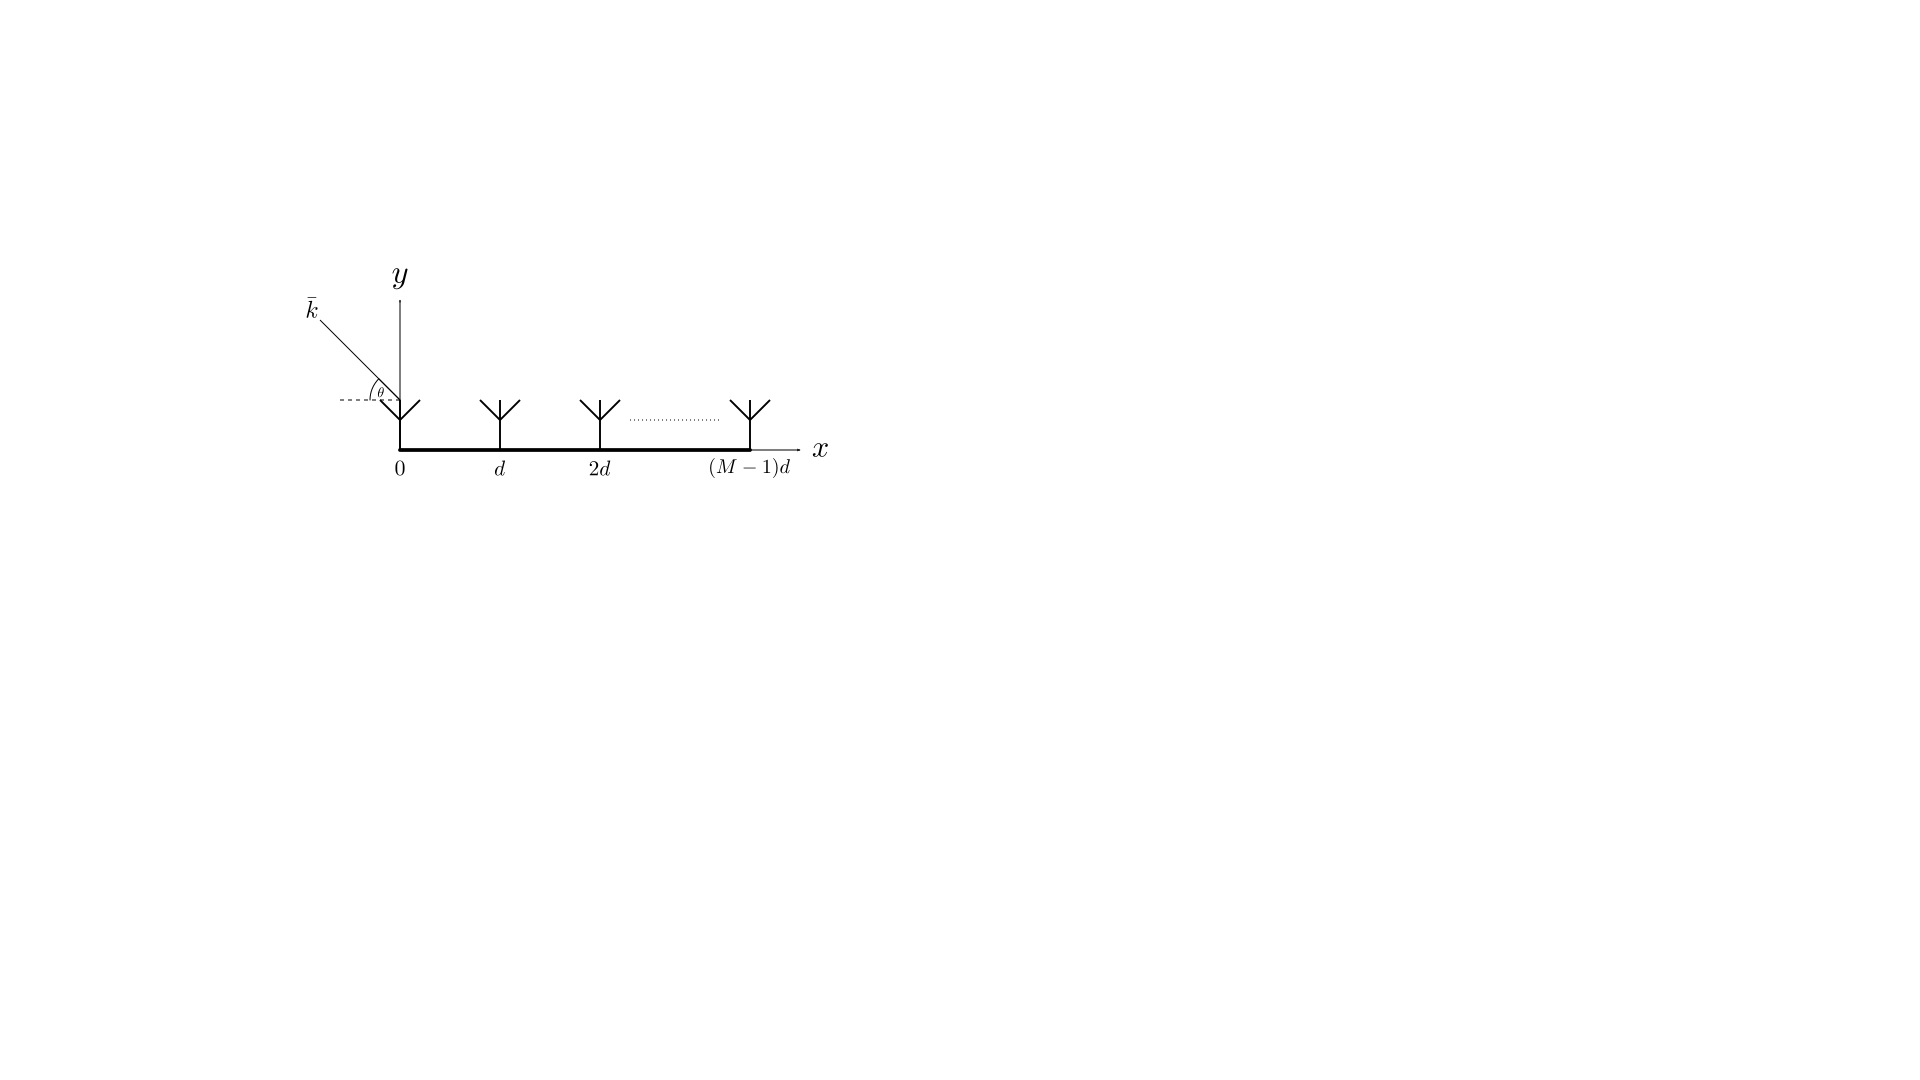
\includegraphics[width=0.7\linewidth]{images/02-Beamforming/ula.png}
    \caption{Arreglo lineal uniforme.}
    \label{fig:beamforming_ula}
\end{figure}

Si tomamos como el ángulo de arribo al indicado por la figura el vector de apuntamiento queda definido por:

\begin{equation}
    \bar{a}_{ALU}(\theta) = g(\theta) \cdot \begin{bmatrix}
        1 & e^{-jkd\cos \theta} & \cdots & e^{-j(M-1)kd \cos \theta}
    \end{bmatrix}
\end{equation}
donde $g(\theta)$ es la ganancia de cada elemento del arreglo en la dirección $\theta$ si consideramos que todos los elementos son idénticos.

\subsubsection{Arreglo circular uniforme}

Como su nombre lo indica, los arreglos circulares uniformes (ACU) consisten en disponer los elementos sobre una circunferencia, equidistante uno del otro, como se muestra en la Figura \ref{fig:beamforming_uca}. Esta disposición bidimensional permite el escaneo tanto en elevación como en azimut de las señales arribantes, y tienen la ventaja de que, por su simetría, permiten que el patrón de radiación sintetizado pueda ser rotado azimutalmente sin sufrir variaciones en su forma \cite{Ucasmartantennas_p193}.

Para el caso bidimensional podemos definir al vector de onda $\bar{k}$ correspondiente a la señal que arriba al arreglo en función del ángulo de elevación y el azimut como:

\begin{equation}
    \bar{k} = k \begin{pmatrix}
        \cos(\theta)\cdot \cos(\varphi) & \cos(\theta)\cdot \sin(\varphi)
    \end{pmatrix}
    \label{eq:beamforming_k}
\end{equation}

El vector $\bar{r}_m$ considerando como origen de coordenadas el centro de la circunferencia que contiene al arreglo puede definirse como:

\begin{equation}
    \bar{r}_m = R \begin{pmatrix}
        \cos(\frac{2\pi\cdot m}{M}) & \sin(\frac{2\pi\cdot m}{M})
    \end{pmatrix}
\end{equation}

Entonces el vector de apuntamiento queda definido como:

\begin{equation}
    \bar{a}_{ACU}(\theta,\varphi) = g(\theta,\varphi) \cdot \begin{bmatrix}
        e^{-jkR\cos\theta \cos\varphi} & \cdots & e^{-jkR(\cos(\frac{2\pi \cdot m}{M})\cos\theta\cdot \cos\varphi+\sin(\frac{2\pi \cdot m}{M})\cos\theta\cdot \sin\varphi)}
    \end{bmatrix}
\end{equation}
Debe notarse que ahora la directividad de la antena queda expresada tanto en elevación como en azimut.

\begin{figure}
    \centering
    \begin{subfigure}[b]{0.7\textwidth}
        \centering
        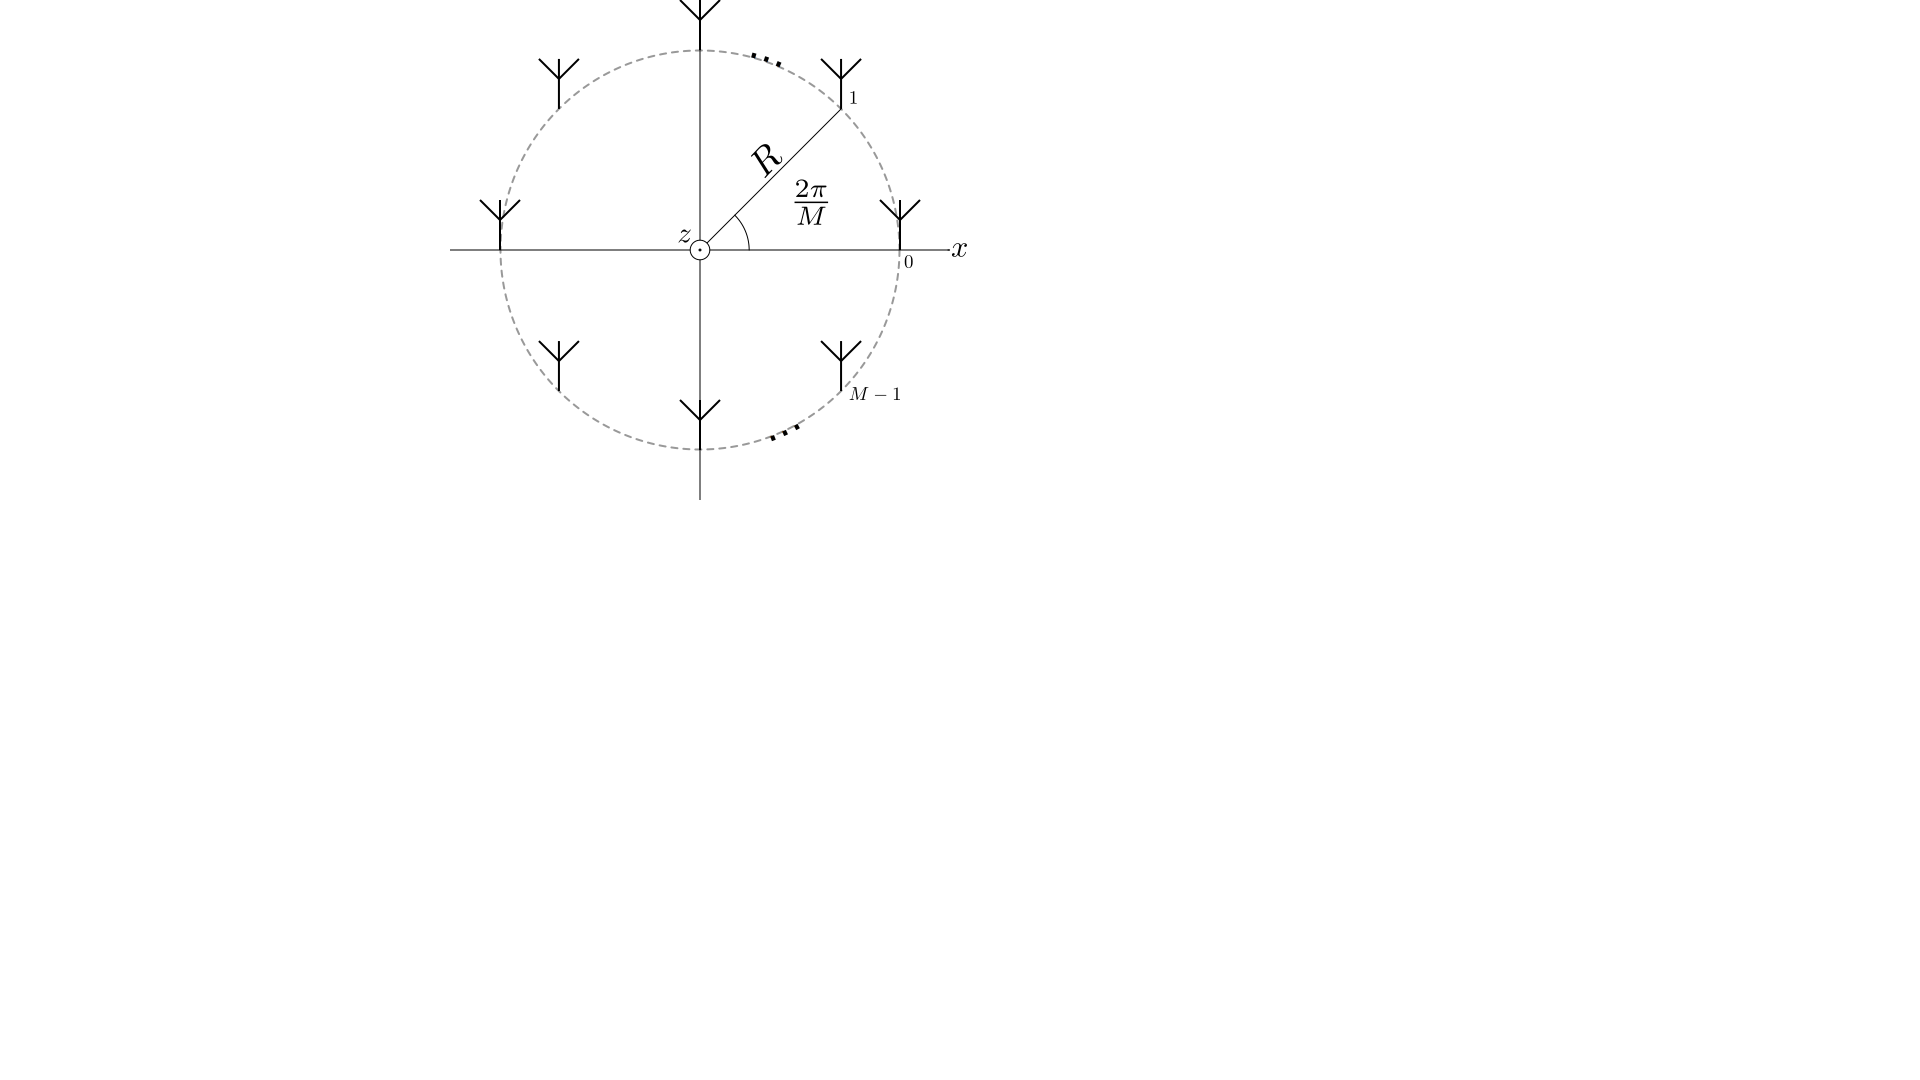
\includegraphics[width=\linewidth]{images/02-Beamforming/uca.png}
    \end{subfigure}
    \hfill
    \begin{subfigure}[b]{0.7\textwidth}
        \centering
        \includegraphics[width=\linewidth]{images/02-Beamforming/uca_3d.png}
    \end{subfigure}
    \caption{Arreglo circular uniforme.}
    \label{fig:beamforming_uca}
\end{figure}


\subsubsection{Arreglo rectangular uniforme}

El arreglo rectangular uniforme (ARU) es el tipo de arreglo de antenas en fase bidimensional más utilizado, debido a que permite contar con la mayor cantidad de elementos en un menor espacio, aumentando la resolución que se puede alcanzar tanto en elevación como azimut. Esta disposición consiste en ubicar a los elementos en una grilla rectangular, manteniendo una misma distancia $d$ cada uno con su adyacente. Un esquema de este tipo de arreglos se muestra en la Figura \ref{fig:beamforming_ura}.

\begin{figure}
    \centering
    \begin{subfigure}[b]{0.6\textwidth}
        \centering
        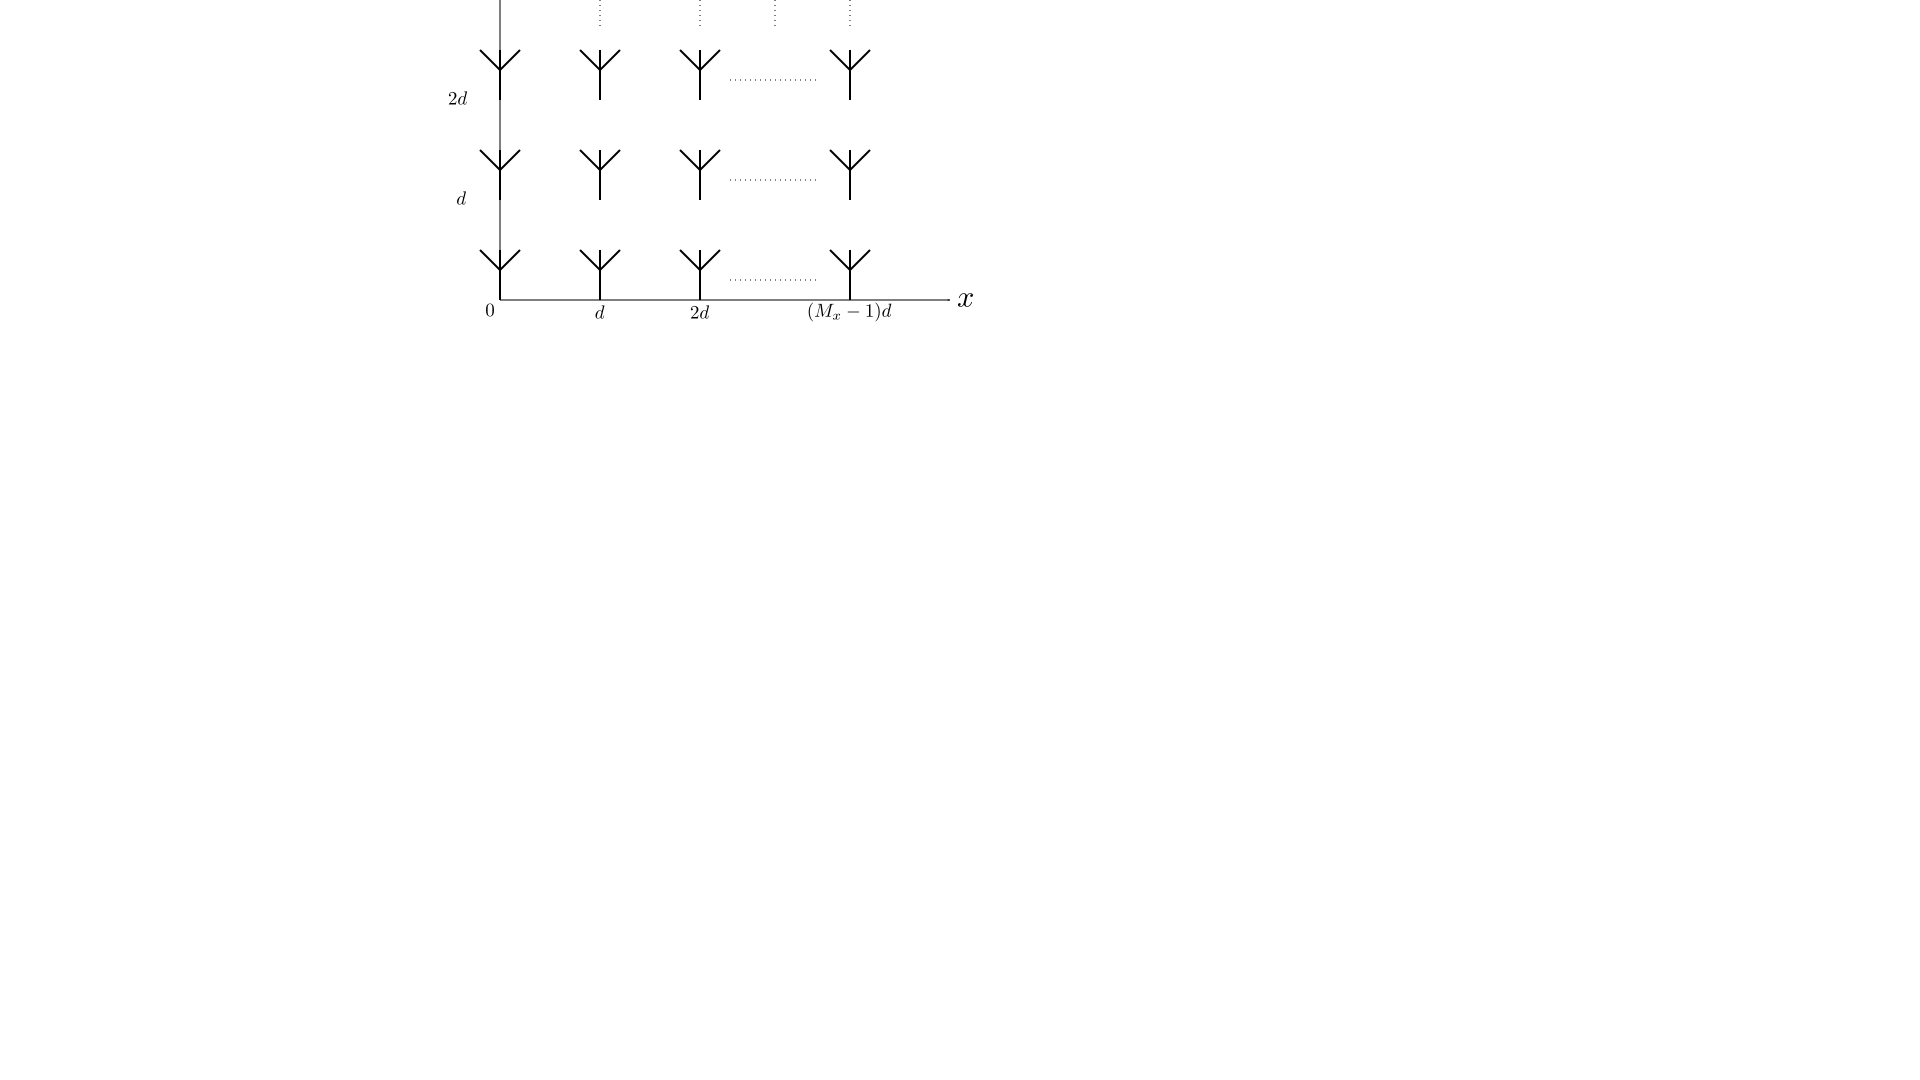
\includegraphics[width=\linewidth]{images/02-Beamforming/ura.png}
    \end{subfigure}
    \hfill
    \begin{subfigure}[b]{0.7\textwidth}
        \centering
        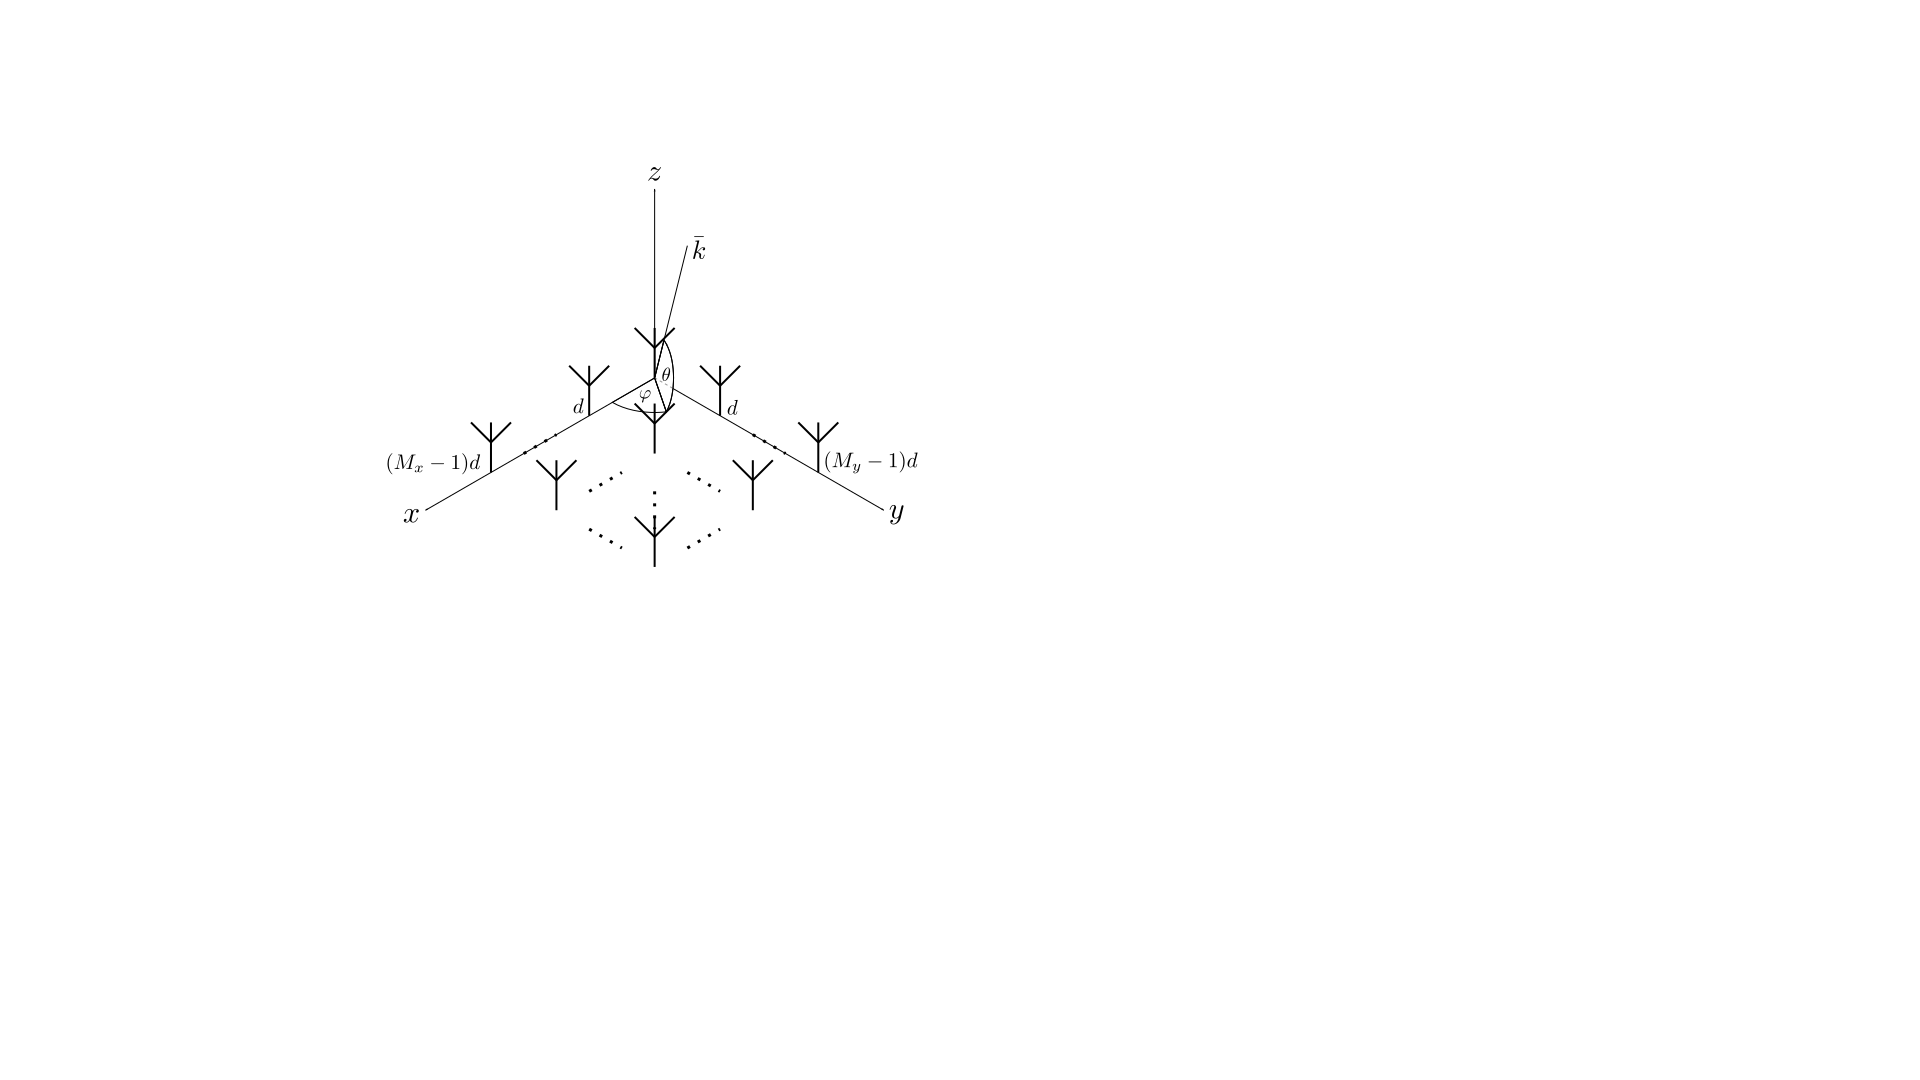
\includegraphics[width=\linewidth]{images/02-Beamforming/ura_3d.png}
    \end{subfigure}
    \caption{Arreglo rectangular uniforme.}
    \label{fig:beamforming_ura}
\end{figure}

El vector $\bar{r}_{m_x,m_y}$ que une al elemento ubicado en las coordenadas $d\cdot(m_x,m_y)$ con el origen de coordenadas, el cual va a estar ubicado en uno de los elementos del extremo del arreglo que se considerará como elemento de referencia, puede definirse como:

\begin{equation}
    \bar{r}_{m_x,m_y} = d \begin{pmatrix}
        m_x & m_y
    \end{pmatrix}
\end{equation}

Debido a que en este caso tenemos un disposición matricial de elementos se debe elegir una convención para identificar a cada elemento del arreglo con una ubicación de un vector. La convención elegida es la de apilar cada una de las columnas a lo largo del eje definido como $y$, de manera que el vector de muestras puede definirse como:

\begin{equation}
    \bar{x}(t)= \begin{bmatrix}
        x_{0,0}(t) & \cdots & x_{0,M_y-1}(t) & \cdots & x_{M_x-1,0}(t) & \cdots & x_{M_x-1,M_y-1}(t)
    \end{bmatrix}
\end{equation}

Teniendo en cuenta lo anterior y utilizando el vector de onda definido en \ref{eq:beamforming_k}, podemos escribir el correspondiente vector de apuntamiento como:

\begin{equation}
    \bar{a}_{ARU}(\theta,\varphi) = g(\theta,\varphi) \cdot \begin{bmatrix}
        1 & \cdots & e^{-jkd[(M_x-1)\cos\theta\cos\varphi+(M_y-1)\cos\theta\sin\varphi]}
    \end{bmatrix}
\end{equation}

El arreglo rectangular uniforme es el tipo de arreglo más importante para el resto de este trabajo ya que es el elegido para realizar la implementación del sistema de conformación de haz que se busca implementar.

\section{Problema a resolver}\label{subc:beamforming_problem}

Según los conceptos que se detallaron a lo largo de esta sección se pueden detallar aún más el objetivo mencionado en la Sección \ref{subc:objetivos} y decir que el objetivo de este proyecto es realizar la implementación de un conformador digital de haz adaptativo para la recepción de señales de satélites LEO utilizando un arreglo de antenas en fase rectangular uniforme de 16 elementos dispuestos en una matriz de 4x4. La señal satelital arriba al arreglo de antenas con una cierta dirección identificada por sus ángulos de elevación y azimut, identificados respectivamente por las letras $\theta$ y $\varphi$. Un esquema de este problema puede verse en la Figura \ref{fig:beamforming_problem}.

\begin{figure}[ht]
    \centering
    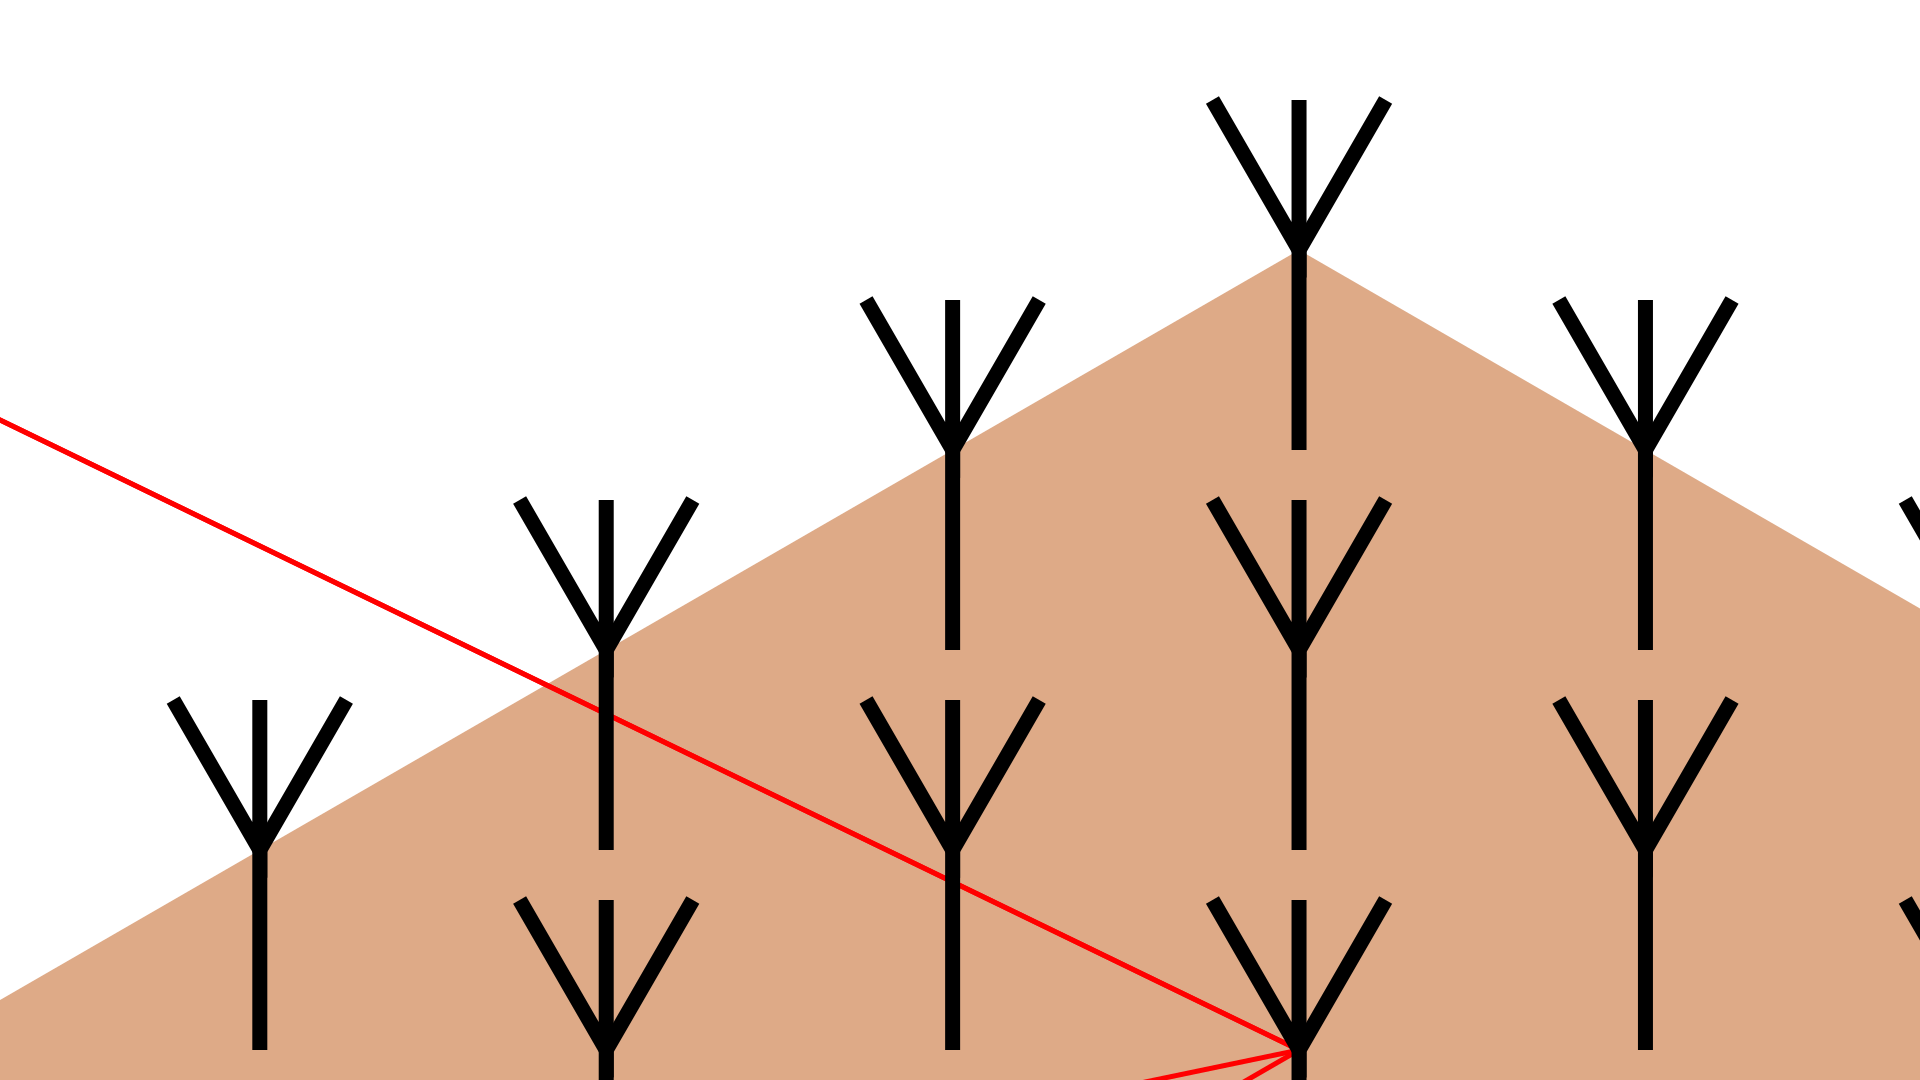
\includegraphics[width=1\linewidth]{images/02-Beamforming/problem.png}
    \caption{Esquema del problema a resolver.}
    \label{fig:beamforming_problem}
\end{figure}

Para realizar la conformación de haz se realizará la estimación de la dirección de arribo utilizando un algoritmo apropiado, el cual brindará esa información al conformador que se encargará de entregar la señal resultante. En la siguiente sección se hará un análisis de dos algoritmos de estimación de dirección de arribo, haciendo hincapié en las comparaciones en el rendimiento y la fiabilidad entre ambos.